% -*- TeX:de -*-
\NeedsTeXFormat{LaTeX2e}
\documentclass[12pt,a4paper,titlepage]{article}

%\usepackage[ngerman]{babel} % german text
\usepackage[DIV12]{typearea} % size of printable area
\usepackage[T1]{fontenc} % font encoding
\usepackage[utf8]{inputenc} % probably on Linux

\usepackage{graphicx} % to include images
\graphicspath{ {img/} } % set default image directory
\usepackage{subfigure} % for creating subfigures
\usepackage{amsmath} % a bunch of symbols
\usepackage{amssymb} % even more symbols
\usepackage{booktabs} % pretty tables
\usepackage{csquotes}

% a floating environment for circuits
\usepackage{float}
\usepackage{caption}

\newfloat{circuit}{tbph}{circuits}
\floatname{circuit}{Schaltplan}

% a floating environment for diagrams
\newfloat{diagram}{tbph}{diagrams}
\floatname{diagram}{Diagramm}

\renewcommand{\familydefault}{\sfdefault} % activate to use sans-serif font as default

\sloppy % friendly typesettings

\usepackage{eurosym}
\usepackage{makeidx}
\usepackage{amsfonts}
\usepackage{mparhack}
\usepackage{array}
\usepackage{tabularx}
\usepackage{minitoc}
\usepackage[colorlinks=true]{hyperref}
\usepackage{epstopdf}
\usepackage{setspace}
\usepackage{csquotes}

\usepackage{float}
\usepackage{circuitikz}

\ctikzset{voltage/distance from line=.5}

\begin{document}

%%%%%%%%%%%%%%%%%%%%%%%%%%%%%%%%
% create title page
%%%%%%%%%%%%%%%%%%%%%%%%%%%%%%%%

\begin{titlepage}

\begin{figure*}[h!]
  
\includegraphics[width=8cm]{TULogo_CMYK}
\end{figure*}

\begin{center}
\vspace*{1.3cm}
{\Huge Elektrotechnische Grundlagen der Informatik\\(LU 182.692)\\}
\vspace{1.7cm}
{\LARGE Protokoll der 1. Laborübung: \enquote{Messtechnik}\\}
\vspace{1.7cm}

% fill in group number and date of lab here
% CHANGE ME!
{\Large Gruppennr.: 22 \hspace{1cm} Datum der Laborübung: 04.05.2017}

% fill in IDs and names here
% CHANGE ME!
\begin{table}[h!]
\centering
\begin{tabular}{|p{3.5cm}|p{3.5cm}|p{6.5cm}|}
\hline \textbf{Matr. Nr.} & \textbf{Kennzahl} & \textbf{Name} \\
\hline
1614835 & & Jan Nausner \\
\hline
1633068 & & David Pernerstorfer \\
\hline
\end{tabular}
\end{table}

\end{center}
\vspace{1.0cm}

\begin{table}[h!]
\begin{tabular}{|l|l|}
\hline \textbf{Kontrolle} & \checkmark \\
\hline stromrichtige Messschaltung & \\
\hline spannungsrichtige Schaltung & \\
\hline Spannungs- Stromteilerschaltung & \\
\hline Superpositionsprinzip & \\
\hline Erste Messung mit Oszilloskop & \\
\hline Arbitrary Waveforms & \\
\hline X/Y-Betrieb & \\
\hline Diodenkennlinie & \\
\hline
\end{tabular}
\end{table}

\end{titlepage}

%%%%%%%%%%%%%%%%%%%%%%%%%%%%%%%%
% start of actual document
%%%%%%%%%%%%%%%%%%%%%%%%%%%%%%%%

\newpage

\setcounter{page}{2}

\section{Innenwiderstand der Messgeräte}

\subsection{Aufgabenstellung}
In dieser Messung müssen die Innenwiderstände der verwendeten Messgeräte durch geeignete Aufbauten bestimmt werden.

\subsection{Innenwiderstand des Amperemeters}

\subsubsection{Verwendete Materialien und Einstellungen:}
\begin{itemize}
  \item Netzteil: Agilent U8031A
  \item Versorgungsspannung: $1V$
  \item Amperemeter: Amprobe 37XR-A
  \item Voltmeter: Amprobe 37XR-A
  \item Vorwiderstand: $1k\Omega$ (gemessen $0,983k\Omega$), $P_{tot} = \frac{1}{4}W$
\end{itemize}

\subsubsection{Schaltungsaufbau}
\begin{figure}[H]
  \centering
  \begin{circuitikz}[european] \draw
    (-0.2,0) -- (0.2,0)
    (0,0) to[V, v<=$U_Q$] (0,2)
    to[R, l=$1k\Omega$] (2,2)
    to[ammeter, i_=$I_A$, *-*, v^>=$U_A$] (6,2)
    (2,2) -- (2,0) to[voltmeter] (6,0) -- (6,2)
    (6,2) -- (6.5,2)
    (6.5,1.8) -- (6.5,2.2);
  \end{circuitikz}
  \caption{Messung $R_A$}
\end{figure}

\subsubsection{Durchführung}
Das Amperemeter wird in Serie zu dem Vorwiderstand (zur Begrenzung des Stroms) geschalten und das Voltmeter parallel zum Amperemeter. An die gesamte Schaltung wird eine Spannung von $1V$ angelegt. Mit dem Voltmeter wird der Spannungsabfall am Amperemeter und mit dem Amperemeter der fließende Strom für die jeweiligen Messbereiche gemessen.

\subsubsection{Ergebnis}
\begin{table}[H]
  \centering
  \begin{tabular}{c|c|c}
    $U_Q$ & $I_A$ & $U_A$ \\
    \hline
    $1V$ & $504,3\mu A$ & $503,3mV$ \\
    \hline
    $5V$ & $5,013mA$ & $56,4mV$ \\
    \hline
    $20V$ & $0,022A$ & $0,7mV$
  \end{tabular}
  \caption{Gemessene Werte}
\end{table}

\noindent Der Innenwiderstand $R_A$ des Amperemeters kann jetzt über das Ohmsche Gesetz berechnet werden: $R_A = \frac{U_A}{I_A}$.

\begin{table}[H]
  \centering
  \begin{tabular}{c|c}
  Messbereich & $R_A$ (gerundet) \\
  \hline
  $\mu A$ & $998\Omega$ \\
  \hline
  $mA$ & $11,25\Omega$ \\
  \hline
  $A$ & $0,032\Omega$
  \end{tabular}
  \caption{Innenwiderstände}
\end{table}

\noindent Der Innenwiderstand bei einem idealen Amperemeter wäre $R_A = 0\Omega$. Dieser Wert ist jedoch nicht zu erreichen, da dies einem Kurzschluss gleichkommen würde. Bei den verschiedenen Messbereichen werden verschiedene Widerstände benötigt, da z.B. bei kleinen Strömen meist große Widerstände zum Einsatz kommen, wohingegen bei großen Strömen die Widerstände meist klein sind. So wird sichergestellt, dass die Messergebnisse so gering wie möglich verfälscht werden. Trotzdem muss man sich bei Messungen der ohmschen Eigenschaft des Amperemeters und derer möglichen Auswirkungen bewusst sein.

\subsection{Innenwiderstand des Voltmeters}

\subsubsection{Verwendete Materialien und Einstellungen:}
\begin{itemize}
  \item Netzteil: Agilent U8031A
  \item Versorgungsspannung: $20V$
  \item Amperemeter: Amprobe 37XR-A
  \item Voltmeter: Amprobe 37XR-A
\end{itemize}

\subsubsection{Schaltungsaufbau}
\begin{figure}[H]
  \centering
  \begin{circuitikz}[european] \draw
    (0,0) -- (0,-0.5)
    (-0.2,-0.5) -- (0.2,-0.5)
    (0,0) to[V, v<=$U_Q$] (2,0)
    to[ammeter, i=$I_V$] (4,0)
    to[voltmeter] (6,0)
    (6,0) -- (6,-0.5)
    (5.8,-0.5) -- (6.2,-0.5);
  \end{circuitikz}
  \caption{Messung $R_V$}
\end{figure}

\subsubsection{Durchführung}
Das Amperemeter und das Voltmeter werden in Serie geschalten und an die gesamte Schaltung wird eine Spannung von $20V$ angelegt. Mit dem Amperemeter wird der fließende Strom gemessen. Das gewählte Voltmeter hat nur einen Messbereich.

\subsubsection{Ergebnis}
\begin{table}[H]
  \centering
  \begin{tabular}{c|c}
    $U_Q$ & $I_V$ \\
    \hline
    $20V$ & $2,25\mu A$
  \end{tabular}
  \caption{Gemessener Wert}
\end{table}

\noindent Der Innenwiderstand $R_V$ des Voltmeters kann jetzt über das Ohmsche Gesetz berechnet werden: $R_V = \frac{U}{I_V} = \frac{20V}{2,25\mu A} \approx 8,9M\Omega$

\noindent Der Innenwiderstand bei einem idealen Voltmeter wäre $R_V = \infty\Omega$. Dieser Wert ist jedoch nicht zu erreichen, da dies einer Unterbrechung gleichkommen würde. Bei Messungen muss man sich der ohmschen Eigenschaft des Voltmeters und derer möglichen Auswirkungen bewusst sein.

\section{Belastungsfehler}

\subsection{Aufgabenstellung}
Die Werte der gegebenen Widerstände sollen jeweils mittels sowohl spannungsrichtiger und stromrichtiger Schaltung als auch per Direktmessung mit dem Multimeter bestimmt werden. Weiters sollen die unterschiedlichen Messbereiche verwendet werden.

\subsection{Verwendete Materialien und Einstellungen:}
\begin{itemize}
  \item Netzteil: Agilent U8031A
  \item Amperemeter: Amprobe 37XR-A
  \item Voltmeter: Amprobe 37XR-A
  \item diverse Widerstände (siehe Tabelle)
\end{itemize}

\begin{figure}[H]
  \centering
  \label{Figure2.2.1}
  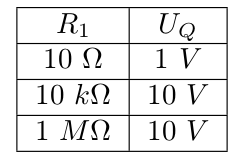
\includegraphics[width=40mm]{widerstandtabelle.png}
  \caption{Widerstände und Quellspannungen}
\end{figure}

\subsection{Schaltungsaufbau}

\begin{figure}[H]
  \centering
  \label{Figure2.3.1}
  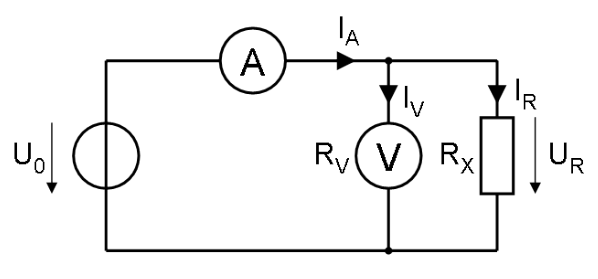
\includegraphics[width=100mm]{spannungsrichtig.png}
  \caption{Spannungsrichtige Messung}
\end{figure}

\begin{figure}[H]
  \centering
  \label{Figure2.3.2}
  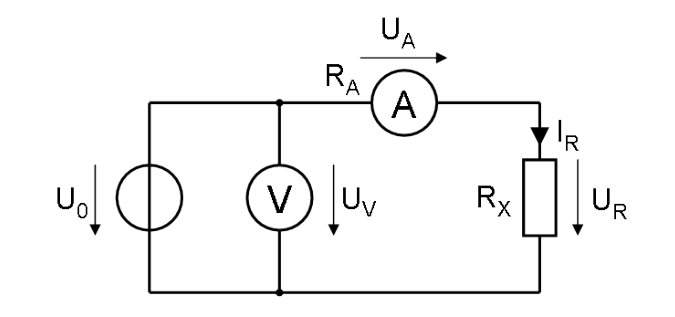
\includegraphics[width=100mm]{stromrichtig.png}
  \caption{Stromrichtige Messung}
\end{figure}


\subsection{Durchführung}
Es wird jeweils die Strom- bzw. Spannungsrichtige Schaltung aufgebaut. Für jeden Widerstand wird die jeweilige Quellspannung eingestellt, danach werden die Werte am Volt- und Amperemeter abgelesen (auch bei unterschiedlichen Messbereichen). Zum Schluss erfolgt noch eine Direktmessung der Widerstände mittels Ohmmeter.

\subsection{Ergebnis}
\begin{table}[H]
  \centering
  \label{Figure2.5.1}
  \begin{tabular}{c|c|c|c}
    $U_0$ & $R_1$ & $U_R$ & $I_A$ \\
    \hline
    $1V$ & $10\Omega$ & $454,2mV$ & $46,16mA$ \\
    \hline
    $1V$ & $10\Omega$ & $983,7mV$ & $0,1A$ \\
    \hline
    $10V$ & $10k\Omega$ & $9,062V$ & $924,9\mu A$ \\
    \hline
    $10V$ & $10k\Omega$ & $9,975V$ & $1,016mA$ \\
    \hline
    $10V$ & $1M\Omega$ & $9,975V$ & $11,22\mu A$ \\
    \hline
    $10V$ & $1M\Omega$ & $9,986V$ & $0,01mA$
  \end{tabular}
  \caption{Spannungsrichtige Messergebnisse}
\end{table}

\begin{table}[H]
  \centering
  \label{Figure2.5.2}
  \begin{tabular}{c|c|c|c}
    $U_0$ & $R_1$ & $U_V$ & $I_R$ \\
    \hline
    $1V$ & $10\Omega$ & $0,999V$ & $38,36mA$ \\
    \hline
    $1V$ & $10\Omega$ & $0,999V$ & $0,1A$ \\
    \hline
    $10V$ & $10k\Omega$ & $9,986V$ & $924,1\mu A$ \\
    \hline
    $10V$ & $10k\Omega$ & $9,986V$ & $1,015mA$ \\
    \hline
    $10V$ & $1M\Omega$ & $9,987V$ & $10,15\mu A$ \\
    \hline
    $10V$ & $1M\Omega$ & $9,986V$ & $0,009mA$
  \end{tabular}
  \caption{Stromrichtige Messergebnisse}
\end{table}

\noindent Die Berechnung des gemessenen Widerstandes $R_m$ mithilfe der spannungsrichtigen Schaltung wird über das ohmsche Gesetz durchgeführt:

\begin{figure}[H]
  \centering
  \label{Figure2.5.3}
  $R_m = \frac{U_R}{I_A}$
\end{figure}

\noindent Um den echten Widerstand $R_x$ zu berechnen, muss man berücksichtigen, dass der gemessene Strom verfälscht ist, da das Voltmeter mit dem Widerstand einen Stromteiler bildet ("spannungsrichtig"). Daraus ergibt sich folgende Formel:

\begin{figure}[H]
  \centering
  \label{Figure2.5.4}
  $R_X = \frac{U_R}{I_R} = \frac{U_R}{I_A-I_V} = \frac{U_R}{I_A-(U_R/R_V)}$
\end{figure}

\noindent Die Berechnung des gemessenen Widerstandes $R_m$ mithilfe der stromrichtigen Schaltung wird über das ohmsche Gesetz durchgeführt:

\begin{figure}[H]
  \centering
  \label{Figure2.5.5}
  $R_m = \frac{U_V}{I_R}$
\end{figure}

\noindent Um den echten Widerstand $R_X$ zu berechnen, muss man berücksichtigen, dass die gemessene Spannung verfälscht ist, da das Amperemeter mit dem Widerstand einen Spannungsteiler bildet ("stromrichtig"). Daraus ergibt sich folgende Formel:

\begin{figure}[H]
  \centering
  \label{Figure2.5.6}
  $R_X = \frac{U_R}{I_R} = \frac{U_V-U_A}{I_R} = \frac{U_V-(R_A*I_R)}{I_R}$
\end{figure}

\begin{table}[H]
  \centering
  \label{Figure2.5.7}
  \begin{tabular}{c|c|c|c}
    $R_{nominell}$ & $R_{spannungsrichtig}$ & $R_{stromrichtig}$ & $R_{Multimeter}$ \\
    \hline
    $10\Omega$ & $9,83\Omega$ & $26\Omega$ & $9,8\Omega$ \\
    \hline
    $1k\Omega$ & $9,82k\Omega$ & $10,8k\Omega$ & $9,82k\Omega$ \\
    \hline
    $1M\Omega$ & $0,89M\Omega$ & $0,98M\Omega$ & $985,5k\Omega$
  \end{tabular}
  \caption{Auswertung der Messergebnisse (gerundet)}
\end{table}

\noindent Etwaige Abweichungen entstehen möglicherweise durch Ungenauigkeiten der Messgerät, aber auch durch Ungenauigkeiten bei den Widerstandswerten. Bei Variante 1 muss die Versorgungsspannung auf $1V$ reduziert werden, da sonst ein zu starker Strom durch den Widerstand fließen würde (z.B. bei $10V\;1A$, was eine Leistung von $10W$ ergeben würde!). Wenn man den Messbereich des Multimeters verstellt, erkennt man, dass manche Messbereiche zu ungenau (out of range oder overflow) sein können.\\
Anhand der Ergebnisse kann man deutlich erkennen, dass die spannungsrichtige Messung für kleine Widerstände (bis zu $k\Omega$) genauer und daher besser geeignet ist, da das Voltmeter hier aufgrund seines hohen Innenwiderstandes den gemessenen Strom kaum verfälscht. Für höhere Widerstandswerte ist die stromrichtige Messung genauer, da hier der geringe Innenwiderstand des Amperemeters keine große Verfälschung der Spannung verursacht.



\section{Spannungs- und Stromteiler}

\subsection{Aufgabenstellung}
Die Spannungs- und Stromteilerregel ist ein wesentlichen Bestandteil der Schaltungsanalyse. In dieser Aufgabe sollen Str\"ome und Spannungen einer einfachen Schaltung (Abbildung~\ref{Figure3.3.2}) berechnet werden. Anschlie\ss end soll diese Schaltung auf einem Steckbrett aufgebaut und die Str\"ome und Spannungen gemessen werden. Die berechneten Werte sollen verifiziert werden, indem sie mit den Messwerten gegen\"ubergestellt werden.

\subsection{Verwendete Materialien und Einstellungen}

\subsection{Theoretische \"Uberlegung}
In der Angabe sind 3 Varianten von Widerst\"anden (Abbildung~\ref{Figure3.3.1}) gegeben. Es soll die Sinnvollste gew\"ahlt werden.
\begin{table}[H]
\centering
\begin{tabular}{|c|c|c|c|c|}
\hline
Variante & $R_1$  & $R_2$  & $R_3$  & $U_0$  \\ \hline
A        & $22 k\Omega$  & $33 k\Omega$  & $27 k\Omega$ & $10 V$ \\ \hline
B        & $22 k\Omega$  & $33 k\Omega$  & $27 k\Omega$  & $10 V$ \\ \hline
C        & $22 k\Omega$  & $33 k\Omega$  & $27 k\Omega$  & $10 V$ \\ \hline
\end{tabular}
\caption{Parameter f\"ur Spannungs- und Stromteiler}
\label{Figure3.3.1}
\end{table}
Bei Variante \textit{A} sind die Widersta\"nde sehr klein, wodurch die thermische Belastbarkeitsgrenze ($P_{tot} < \frac{1}{4} W$) \"uberschritten wird. Bei Variante \textit{C} wird der zu messende Strom sehr gering (im $\mu A$ Bereich), wodurch das Messergebnis ungenau wird. Daher wird Variante \textit{B} gew\"ahlt.

\subsection{Schaltungsaufbau}
\begin{figure}[H]
\centering
\begin{circuitikz}[european]
  \draw
    (0,6) to [V, v=$U_0$] (0,0);
  \draw
    (0,6) to [short, - ,i=$I_1$] (3,6)
    to [R, l=$R_1$, v=$U_1$](3,3)
    to [short, -, i=$I_3$] (3, 2.5)
    to [R, l=$R_2$, v=$U_2$](3,0)
    to [short, *-](0,0);
  \draw
    (3,3) to [short, *-] (5,3)
    to [short, -, i=$I_3$] (5, 2.5)
    to [R, l=$R_3$, v=$U_3$] (5,0)
    to [short, -](3,0);
\end{circuitikz}
\caption{Schaltung Spannungs- und Stromteiler}
\label{Figure3.3.2}
\end{figure}

\subsection{Berechnung Spannungen und Str\"ome}
Da die Aufgabe vorsieht, die Spannungen und Str\"ome der Schaltung mit den gemessen Widerstandswerten zu berechnen, wird hier der Rechenweg erkl\"autert.
\begin{align*}
  R_{ges} &= R_1 + \frac{R_2*R_3}{R_2 + R_3}\\
  I_{1} &= \frac{U_0}{R_{ges}}\\
  U_{1} &= I_1 * R_1\\
  U_{2} &= U_{3} = U_0 - U_1\\
  I_2 &= \frac{U_2}{R_2}\\
  I_3 &= \frac{U_3}{R_3}\\
\end{align*}

\subsection{Durchf\"uhrung}
\begin{itemize}
  \item Die Widerstandswerte der Widerst\"ande werden mit dem Ger\"at mit der Ohmmeter Einstellung gemessen. Die Messergebnisse sind in Abbildung~\ref{Figure3.3.3} zu finden.
  \item Die Spannungen $U_1$, $U_2$ und $U_3$ sowie die Str\"ome $I_1$, $I_2$ und $I_3$ werden berechnet. Dazu werden die gemessenen Widerstandswerte ber\"ucksichtigt. Die berechneten Werte sind in Abbildung~\ref{Figure3.3.4} zu finden.
  \item Die Spannungen werden mit dem Ger\"at XXX mit der Einstellung \textit{Gleichspannung} parallel zu den Widerst\"anden gemssen.
  \item Die Str\"ome werden mit dem Ger\"at XXX mit der Einstellung \textit{mA} (Milli-Ampere) gemessen. Die Messwerte sind in Abbildung~\ref{Figure3.3.4} zu finden.
\end{itemize}

\subsection{Ergebnisse}
\begin{table}[H]
  \centering
  \begin{tabular}{|l|c|c|}
  \hline
     & Widerstandswert lt. Farbcode & gemessener Widerstandswert \\ \hline
  $R_1$ & $22 k\Omega$                    & $21,75 k\Omega$               \\ \hline
  $R_2$ & $33 k\Omega$                    & $32,53 k\Omega$               \\ \hline
  $R_3$ & $47 k\Omega$                    & $46,72 k\Omega$               \\ \hline
  \end{tabular}
  \caption{Messung der Widerst\"ande mit Ohmmeter}
  \label{Figure3.3.3}
\end{table}

\begin{table}[H]
  \centering
  \begin{tabular}{|c|c|c|}
  \hline
  ~  & Spannung berechnet & Spannung gemessen \\ \hline
  $U_1$ & $5,31 V$             & $5,300 V$            \\ \hline
  $U_2$ & $4,69 V$             & $4,673 V$            \\ \hline
  $U_3$ & $4,69 V$             & $4,673 V$            \\ \hline
  \end{tabular}
  \begin{tabular}{|c|c|c|}
  \hline
  ~  & Strom berechnet & Strom gemessen \\ \hline
  $I_1$ & $244,3 \mu A$       & $238,50 \mu A$     \\ \hline
  $I_2$ & $144,04 \mu A$      & $141,10 \mu A$     \\ \hline
  $I_3$ & $99,67 \mu A$       & $98,49 \mu A$      \\ \hline
  \end{tabular}
  \caption{Vergleich Berechnung und Messung der Str\"ome und Spannungen}
  \label{Figure3.3.4}
\end{table}

\subsection{Diskussion}
\subsubsection{Messwerte der Widerst\"ande}
Die gemessenen Widerstandswerte sind nicht exakt, jedoch liegen die Messwerte in der jeweilig angegebenen Toleranzgrenze. An anderer Faktor f\"ur die Abweichung vom eigentlichen Widerstandswert ist die Ungenauigkeit des Ger\"ates XXX, welches lt. Spezifikation bis $1k \Omega$ eine Toleranz von $\pm0.5\%$ bzw. bis $10 M\Omega$ eine Toleranz von $\pm1.0\%$ hat.

\subsubsection{Unterschied berechnete und gemessene Spannungen und Str\"ome}
Der Unterschied zwischen berechneten und gemessen Spannungen und St\"omen ist auf die Messtoleranz des Messger\"ats zur\"uckzuf\"uhren.


\pagebreak
\section{Superpositionsprinzip}
\subsection{Aufgabenstellung}
In dieser Mess\"ubung soll das Superpositionsprinzip verifiziert werden.

\subsection{Theoretische \"Uberlegung}
Das Superpositionsprinzip wird verwendet um Schaltkreise mit mehreren Spannungs- und Stromquellen zu berechnen. Die Berechnung der Spannungen und Str\"ome erfolgt f\"ur jede Quelle getrennt. Dabei werden alle anderen Quelle von der Schaltung getrennt und kurzgeschlossen. Danach werden die Teilergebnisse \"uberlagert, das hei\"st die St\"ome und Spannungen werden jeweils summiert.

\subsection{Berechnung}
Die Spannungen und die Str\"ome werden f\"ur die Schaltung aus Abbildung \ref{Figure4.1.1} berechnet. Hierbei wird eine ideale Spannungsquelle mit Innenwiderstand $0 \Omega$ angenommen.
\begin{table}[H]
\centering
\begin{tabular}{|l|l|l|}
\hline
                                  & Spannung $U_{RX}$ & Strom $I_{RX}$     \\ \hline
Stromquelle $U_1$ kurzgeschlossen & $0,33 V$ & $331,92 \mu A$ \\ \hline
Stromquelle $U_2$ kurzgeschlossen & $2,55 V$   & $2,55 mA$   \\ \hline
Summe                             & $2,88 V$  & $2,88 mA$ \\\hline
\end{tabular}
\caption{Berechnung der Schaltung mittels Superpositionsprinzip}
\label{Figure4.1.1}
\end{table}

\subsection{Schaltungsaufbau}
\begin{figure}[H]
\centering
\begin{circuitikz}[european]
  \draw
    (0,4) to [V, v=$U_0$] (0,0);
  \draw
    (0,4) to [R, l=$R_1$] (3,4);
  \draw
    (3,4) to [R, l=$R_2$] (3,0)
    (3,0) to [short, *-] (0,0);
  \draw
    (3,4) to [short, *-] (3,4.5);
  \draw
    (3,4.5) to [R, l=$R_2$] (7,4.5);
  \draw
    (7,4.5) to [short, -*] (7,4);
  \draw
    (7,4) to [R, l=$R_4$] (7,0);
  \draw
    (7,0) to [short, *-] (3,0);
  \draw
    (7,4) to [V, v=$U_2$] (10,4);
  \draw
    (10,4) to [R, l=$R_5$] (10,0);
  \draw
    (10,0) to [short,-] (7,0);
  \draw
    (7,4) to [R, l=$R_x$, v=$U_x$, i=$I_x$] (3,0);
\end{circuitikz}
\caption{Schaltungsaufbau}
\label{Figure4.2.1}
\end{figure}

\subsection{Durchf\"uhrung}
\begin{enumerate}
  \item Die Schaltung aus Abbildung wird auf einem Steckbrett aufgebaut.
  \item Die Schaltung wird von der Spannungsquelle $U_2$ getrennt und kurzgeschlossen.
  \item Die Schaltung wird mit dem Netzteil XXX verbunden.
  \item Auf dem Ger\"at wird eine Spannung von $10 V$ eingestellt.
  \item Die Spannungsmessung erfolgt mit dem Ger\"at XXX mit der Einstellung XXX.
  \item Die Spannung wird parallel zum Widerstand $R_X$ gemessen.
  \item Der Strom wird in Serie mit dem Widerstand $R_X$ gemessen.
  \item Die gleichen Messungen erfolgen analog mit der Spannungsquelle $U_1$ kurzgeschlossen und mit beiden Spannungsquellen angeschlossen.
  \item Die Messwerte sind in Abbildung~\ref{Figure4.4.5} zu finden.
\end{enumerate}

\subsection{Ergebnisse}
\begin{table}[H]
\centering
\begin{tabular}{|l|l|l|}
\hline
                                 & Spannung $U_{R_X}$ & Strom $I_{R_X}$      \\ \hline
Stromquelle $U_1$ kurzgeschlossen & $2,541 V$    & $2,611 mA$     \\ \hline
Stromquelle $U_2$ kurzgeschlossen & $330,9 mV$   & $237,9 \mu A$ \\ \hline
beide Stromquellen angeschlossen  & $2,872 V$    & $2,901 mA$ \\ \hline
\end{tabular}
\caption{Strom und Spannungsmessung am Widerstands $R_X$}
\label{Figure4.4.5}
\end{table}

\subsection{Diskussion}
Bei der Messung des Stromes am Widerstand $R_X$ ergibt sich im Vergleich \textit{Summe Spannungsmesswerte mit jeweils einer Stromquelle getrennt} zu \textit{Spannungsmessung mit beiden Stromquellen aktiv} eine Differenz von $51 \mu A$. Dies ist mit der Messtoleranz des Amperemeters zu begr\"unden, welches lt. Spezifikation eine Messtoleranz von $\pm0.5\%$ bei der Einstellung \textit{2m} hat. \\
Bei dem gleichen Gegen\"uberstellung im Bezug auf die Spannung wurde keine Abweichung festgestellt.


\section{Erste Messung mit Oszilloskop}
\subsection{Aufgabenstellung}
In dieser Mess\"ubung soll der Umgang mit Ozsillskop und Frequenzgenerator ge\"ubt werden. Dazu soll eine einfache Schaltung aufgebaut und ein Signale erzeugt und gemessen werden.

\subsection{Schaltungsaufbau}
\begin{figure}[H]
\centering
\begin{circuitikz}[european]
  \draw (0,2) to [short, ->, l=$Frequenzgenerator$](4,2);
  \draw (4,2) node[inputarrow] {};
  \draw (8,2) to [short, ->, l=$Oszilloskop$](12,2);
  \draw (12,2) node[inputarrow] {};
  \draw (2,4) to [short, -] (6,4);
  \draw (6,4) to [R=100<\kilo\ohm>, l={$R_1 100k\Omega$}] (6,0);
  \draw (6,0) to [short, -] (2,0);
  \draw (6,3.5) to [short, *-] (9,3.5);
  \draw (6,0.5) to [short, *-] (9,0.5);
\end{circuitikz}
\caption{Oszilloskop und Frequenzgenerator}
\label{Figure3.5.1}
\end{figure}

\subsection{Verwendete Materialien und Ger\"ate}

\subsection{Berechnung}
In der Angabe ist eine Frequenz von $5,27 MHz$ angegeben. Da am Funktionsgenerator f\"ur die Funktionsart $Square$ nur die Periodendauer eingestellt werden kann, wird diese berechnet.\\
\begin{equation}
T = \frac{1}{5,27 MHz} \approx 190 ns
\end{equation}

\subsection{Durchf\"uhrung}
\begin{itemize}
  \item Die Schaltung aus Abbildung \ref{Figure3.5.1} wird auf einem Steckbrett aufgebaut.
  \item Am Funktionsgenerator werden folgende Einstellungen vorgenommen:
    \begin{enumerate}
      \item Funktionsart: Rechteck (Taste $Square$)
      \item Frequenz: $5,27 MHz \Leftrightarrow \sim190 ns$ (Softkey \textit{Freq Period})
      \item $3,3 V_{PP}$ (Softkey \textit{Ampl HiLevel})
      \item Offset $1 V$ (Softkey \textit{Offset LoLevel})
      \item Duty Circle $25 \%$ (Softkey \textit{Duty Circle})
      \item Lastimpedanz: HighZ (\textit{Utility} $\rightarrow$ \textit{OUTPUT-Setup})
    \end{enumerate}
  \item Der Funktionsgenerator und das Oszilloskop werden mit der Schaltung lt. Schaltplan verbunden.
  \item Die \textit{Auto-Scale} Taste wird gedr\"uckt. Dadurch wird das Oszilloskop so konfiguriert, dass das Eingangssignal bestm\"oglich dargestellt wird.
  \item Mittels Cursorfunktion wird die Amplitude gemessen. Dazu wird ein Y-Cursor am Minimum und ein Y-Cursor am Maximum angelegt. Es wird jeweils der Abstand des Cursors zur X-Achse angezeigt (Abbildung \ref{Figure3.5.2}).
  \item Mittels Cursorfunktion wird die Periodendauer gemessen. Dazu wird ein X-Cursor am positiven Sprung des Rechtecksignals und ein zweiter X-Cursor an der gleichen Stelle eine Periode sp\"ater angelegt (Abbildung \ref{Figure3.5.2})
  \item Mittels Quick-Measure Funktion werden Effektivwert, Mittelwert und der Pk-Pk-Wert gemessen. Dazu werden folgende Measurements am Oszilloskop hinzugef\"ugt (Softkey \textit{Add Measurement}).
    \begin{enumerate}
      \item Effektivwert: \textit{DC RMS-Cyc.}
      \item Mittelwert: \textit{Avg-Cyc.}
      \item Pk-Pk-Wert: \textit{Pk-Pk}
    \end{enumerate}
    Aus Abbildung \ref{Figure3.5.3} werden die Messwerte abgelesen (Abbildung  \ref{Figure3.5.4}).
  \item Am Funktionsgenerator wird die Lastimpedanz auf $50 \Omega$ ge\"andert (\textit{Utility} $\rightarrow$ \textit{OUTPUT-Setup}).
  \item Am Funktionsgenerator wird unter der Einstellung \textit{Amplitude} nun $V_{PP} = 1,65 V$ angezeigt.
  \item Die Anzeige am Oszilloskop bleibt unver\"andert.
  \item Der $100 k\Omega$ Widerstand wird nun durch einen $50 k\Omega$ Widerstand ausgetauscht.
  \item Mittels Quick-Measure Funktion werden die nochmals die gleichen Messwerte am Oszilloskop gemessen. Aus Abbildung \ref{Figure3.5.5} werden die Messwerte \ref{Figure3.5.4} abgelesen.
\end{itemize}

\subsection{Ergebnisse}
\begin{table}[H]
  \centering
  \begin{tabular}[t]{|l|r|}
  \hline
                     & Spannung {[}V{]} \\ \hline
  0 - pos. Amplitude & $2,46250 V$          \\ \hline
  0 - neg. Amplitude & $-2,56250 V$         \\ \hline
  \end{tabular}
  \begin{tabular}[t]{|l|r|}
  \hline
          & Periodendauer {[}s{]} \\ \hline
  $\Delta Y$ & $190 ns$ \\ \hline
  \end{tabular}
  \caption{Messwerte Amplitude und Periodendauer}
  \label{Figure3.5.2}
\end{table}

\begin{figure}[H]
  \centering
  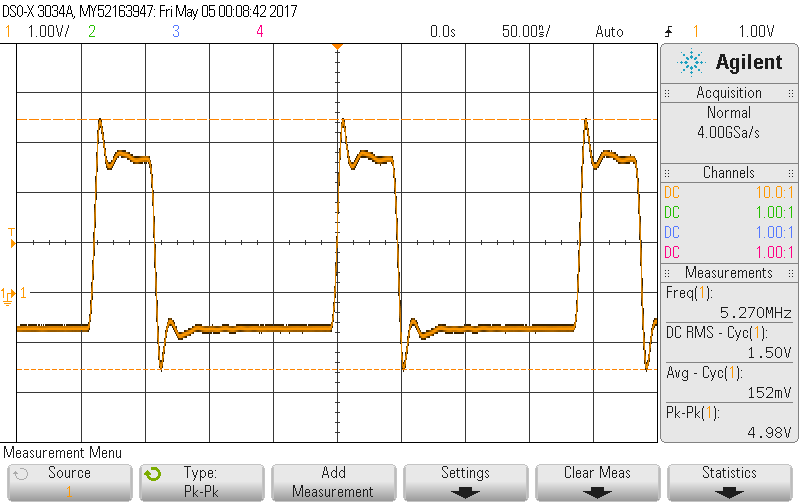
\includegraphics[width=14cm]{oszi_square_100k.png}
  \caption{Oszilloskop Rechtecksignal bei $100 k\Omega$}
  \label{Figure3.5.3}
\end{figure}

\begin{figure}[H]
  \centering
  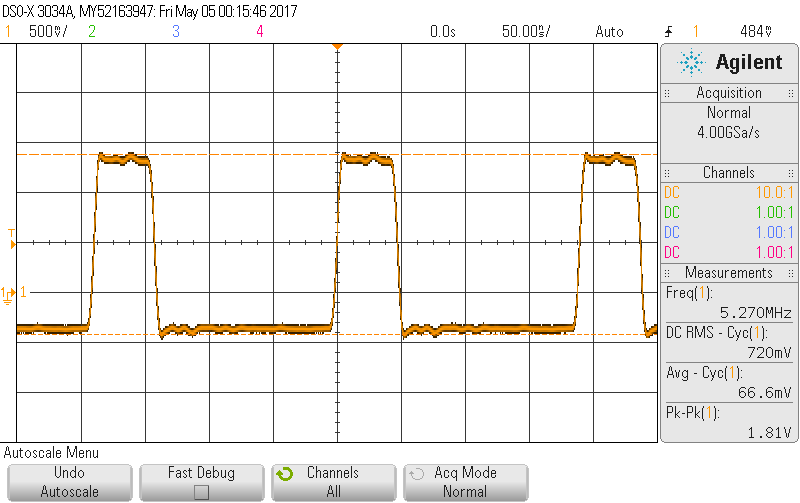
\includegraphics[width=14cm]{oszi_square_50.png}
  \caption{Oszilloskop Rechtecksignal bei $50 \Omega$}
  \label{Figure3.5.5}
\end{figure}

\begin{table}[H]
\centering
\begin{tabular}[t]{|l|r|r|r|}
\hline
           & Effektivwert {[}V{]} & Mittelwert {[}V{]} & Pk-Pk-Wert {[}V{]} \\ \hline
$R_1=100 k\Omega$ & 1,50 V               & 1,49 mV            & 5,03 V             \\ \hline
$R_1=50 \Omega$    & 720 mV               & 70 mV              & 1,83 V             \\ \hline
\end{tabular}
\caption{Messwerte Effektivwert, Mittelwert und Pk-Pk-Wert}
\label{Figure3.5.4}
\end{table}

\subsection{Diskussion}
In Abbildung~\ref{Figure3.5.3} sieht man an der positiven Flanke des Rechtecks eine \"Uberschwingung. Dieses Vehalten wird Gibbsches Ph\"anomen genannt. In der Praxis gibt es keine M\"oglichkeit eine exakte Rechteckfunktion zu erzeugen. Stattdessen wird die Funktion mit \"Uberlagerung von Sinusfunktionen verschiedener Frequenzen m\"oglichst genau approximiert. Die \"Uberschwingung ist ein Nebeneffekt dieser \"Uberlagerung. \\



\section{Arbitrary Waveform}

\subsection{Aufgabenstellung}
In diesem Beispiel soll ein moduliertes Signal durch Überlagerung zwei verschiedener Schwingungen erzeugt und dargestellt werden.

\subsection{Verwendete Materialien und Einstellungen:}
\begin{itemize}
  \item Oszilloskop: Agilent InfiniiVision MSO-X 3054A
  \item Funktionsgenerator: Agilent 33220A
  \item Widerstand: $100k\Omega$
\end{itemize}

\subsection{Schaltungsaufbau}
\begin{figure}[H]
  \centering
  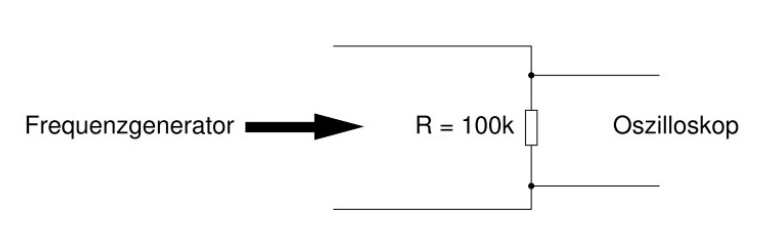
\includegraphics[width=100mm]{oszi_sg.png}
  \caption{Verbindung von Oszilloskop und Funktionsgenerator}
  \label{Figure6.3.1}
\end{figure}

\subsection{Durchführung}
Am Frequenzgenerator (Lastwiderstand \"High Z\") wird zuerst ein Dreieckssignal erzeugt. Dazu wird der Signaltyp \"Ramp\" ausgewählt, eine Freqzenz von $400Hz$ und eine Amplitude von $1V$ eingestellt, sowie die Symmetrie auf 50\% gesetzt (um den Sägezahn in ein Dreieck zu formen). Dann wird dem Dreieckssignal (mit Taste \"Mod\") ein Sinus mit Periodendauer $200\mu s$ ($f = \frac{1}{200\mu s} = 5kHz$) ("AM Freq") und Amplitude $100mV$ ("AM Depth") aufmoduliert. Die Schwingung wird am Oszilloskop dargestellt.

\subsection{Ergebnis}

\begin{figure}[H]
  \centering
  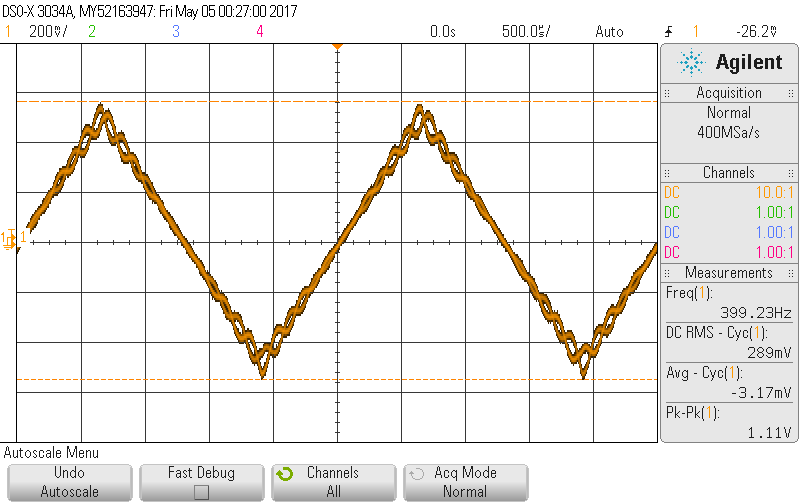
\includegraphics[width=150mm]{moduliertes_signal.png}
  \caption{Moduliertes Signal}
  \label{Figure6.5.1}
\end{figure}



\section{X/Y-Betrieb}

\subsection{Aufgabenstellung}
In dieser Aufgabe soll man sich mit dem X/Y-Betrieb des Oszilloskops vertraut machen.

\subsection{Schaltungsaufbau}
\begin{figure}[H]
\centering
\begin{circuitikz}[european]
  \draw (0,4) to [V, v=$U$] (0,0);
  \draw (0,4) to [short, -] (2,4);
  \draw (2,4) to [R, l=$50 k\Omega$] (2,2);
  \draw (2,2) to [short, *-] (4,2);
  \draw (4,2) to [short, -](4,1) node[ground]{};
  \draw (0,0) to [short, -] (2,0);
  \draw (2,0) to [C, l=$6 \mu 8$] (2,2);
\end{circuitikz}
\caption{Oszilloskop und Frequenzgenerator}
\label{Figure7.3.1}
\end{figure}

\subsection{Verwendete Materialien und Ger\"ate}
BNC Kabel


\subsection{Durchf\"uhrung}
\begin{itemize}
  \item Die Schaltung aus Abbildung~\ref{Figure7.3.1} wird auf einem Steckbrett aufgebaut.
  \item Am Kanal 1 des Oszilloskops wird die Spannung am Widerstand gemessen. Dazu wird der Pluspol des BNC Kabels in der Schaltung zwischen Spannungsquelle und Widerstand verbunden und der Minuspol zwischen Widerstand und Kondensator.
  \item Am Kanal 2 des Oszilloskops wird die Spannung am Kondensator gemessen. Dazu wird er Pluspol des BNC Kabels in der Schaltung zwischen Spannungsquelle und Widerstand verbunden und der Minuspol zwischen Widerstand und Kondensator.
  \item Am Funktionsgenerator werden folgende Einstellungen vorgenommen:
  \begin{itemize}
    \item Funktionsart: Sinus (Taste \textit{Sine})
    \item $5 V_{PP}$ (Softkey \textit{Ampl HiLevel})
    \item Offset $0 V$ (Softkey \textit{Offset LoLevel})
    \item Duty Circle $50 \%$ (Softkey \textit{Duty Circle})
  \end{itemize}
  \item Mit der Taste \textit{Output} am Funktionsgenerator wird die Spannungsquelle aktiviert.
  \item Am Oszilloskop wird ein Signal sichtbar.
  \item Nun wird die Frequenz am Funktionsgenerator so adjustiert, dass die Amplituden der beiden Kan\"ale in etwa gleich gro\ss  sind.
  \item Bei einer Frequenz von $500 Hz$ sind die Amplituden der beiden Signale in etwa gleich gro\ss .
  \item Der Funktionsgenerator wird wie folgt eingestellt.
  \begin{enumerate}
    \item Um in den X/Y-Betrieb zu wechseln, wird die Taste \textit{Horiz.} gedr\"uckt.
    \item Auf der X-Achse wird das Signal von Kanal 1 eingestellt. Au\ss erdem wird hier das Signal invertiert geschalten.
    \item Auf der Y-Achse wird das Signal von Kanal 2 eingestellt.
  \end{enumerate}
  \item Das geometrische Ergebnis dieser Einstellung ist ein Kreis (Abbildung~\ref{Figure7.6.1}).
  \item Die Frequenz wird am Funktionsgenerator erh\"oht ($900 Hz$) und am Oszilloskop etsteht eine in X-Richtung gestreckte Ellipse (Abbildung~\ref{Figure7.6.2}).
  \item Die Frequenz wird am Funktionsgenerator verringert ($300 Hz$) und am Oszilloskop etsteht eine in Y-Richtung gestreckte Ellipse (Abbildung~\ref{Figure7.6.3}).
\end{itemize}

\subsection{Ergebnisse}
\begin{figure}[H]
  \centering
  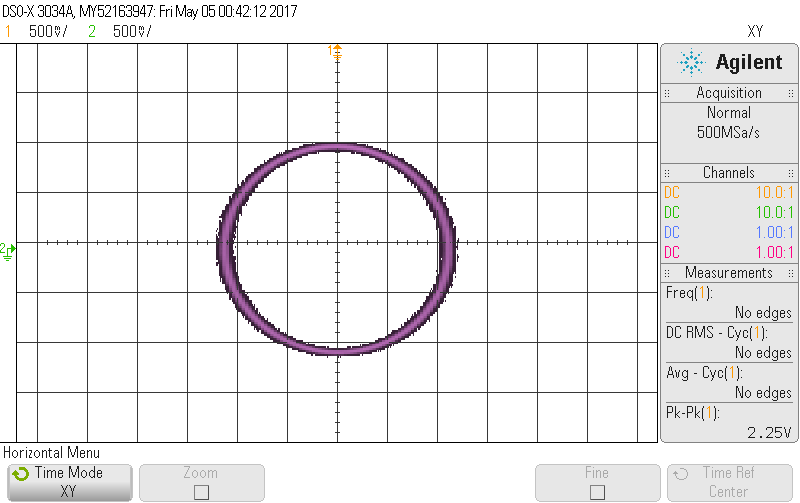
\includegraphics[width=14cm]{oszi_xy_circle_500hz.png}
  \caption{Oszilloskop X/Y-Betrieb bei Frequenz $500 Hz$}
  \label{Figure7.6.1}
\end{figure}
\begin{figure}[H]
  \centering
  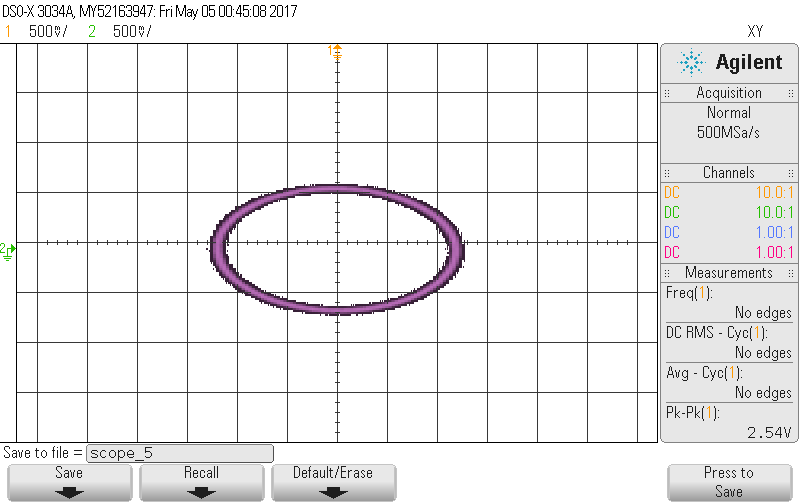
\includegraphics[width=14cm]{oszi_xy_circle_900hz.png}
  \caption{Oszilloskop X/Y-Betrieb bei Frequenz $900 Hz$}
  \label{Figure7.6.2}
\end{figure}
\begin{figure}[H]
  \centering
  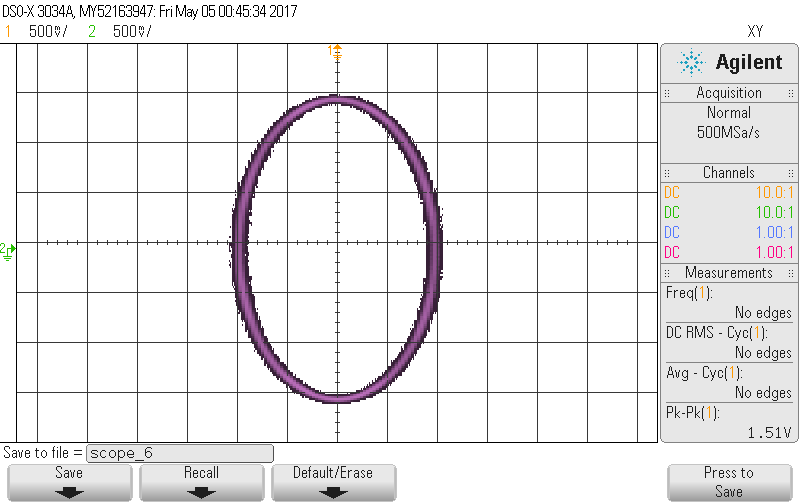
\includegraphics[width=14cm]{oszi_xy_circle_300hz.png}
  \caption{Oszilloskop X/Y-Betrieb bei Frequenz $300 Hz$}
  \label{Figure7.6.3}
\end{figure}

\subsection{Diskussion}
\subsubsection{Entstehung des Kreises}
Hier wird erl\"autert welche geometrische Form durch die gegebene Schaltung am Oszilloskop im X/Y-Betrieb erzeugt wird.\\
Durch die sinusf\"ormige Eingangsspannung entsteht am Widerstand der selbe Spannungsverlauf. Mathematisch betrachtet ergibt sich also die folgende Funktion f\"ur die Spannung am Widerstand.
\begin{align*}
  U_R(t) = A*\sin{t}
\end{align*}
Am Kondensator ergibt sich ebenfalls eine sinusf\"ormige Spannung, jedoch im Bezug zur Eingangsspannung um $90^{\circ}$ verschoben. Mathematisch betrachtet ergibt sich also die folgende Funktion f\"ur die Spannung am Kondensator.
\begin{align*}
  U_C(t) = A*\cos{t}
\end{align*}
Bildet man nun aus den beiden Funktionen einen Graphen, wobei $U_C$ auf der X-Achse und $U_R$ auf der Y-Achse aufgtragen wird, so ergibt sich die geometrische Form eines Kreises.\\
Da $U_C(t)$ mit dem Minuspol der Wechselspannungsquelle verbunden ist, muss die Funktion noch zus\"atzlich invertiert werden.

\subsubsection{\"Anderung der Frequenz}
Bei \"Anderung der Frequenz der Eingangsspannung \"andert sich die Amplitude der Spannung am Kondensator. Dadurch ergibt sich bei erh\"ohung der Frequenz eine Streckung des Kreises in Richtung X-Achse, bei Verringerung der Frequenz ergibt sich eine Streckung in Richtung Y-Achse.


\section{Diodenkennlinie}

\subsection{Aufgabenstellung}
Die Eigenschaften der Diode als nichtlineares Bauelement sollen in Form einer Kennlinier am Oszilloskop dargestellt werden.

\subsection{Verwendete Materialien und Einstellungen:}
\begin{itemize}
  \item Oszilloskop: Agilent InfiniiVision MSO-X 3054A
  \item Funktionsgenerator: Agilent 33220A
  \item Widerstand: $100\Omega$
  \item Dioden: LED rot, 1N4148
\end{itemize}

\subsection{Schaltungsaufbau}
\begin{figure}[H]
  \centering
  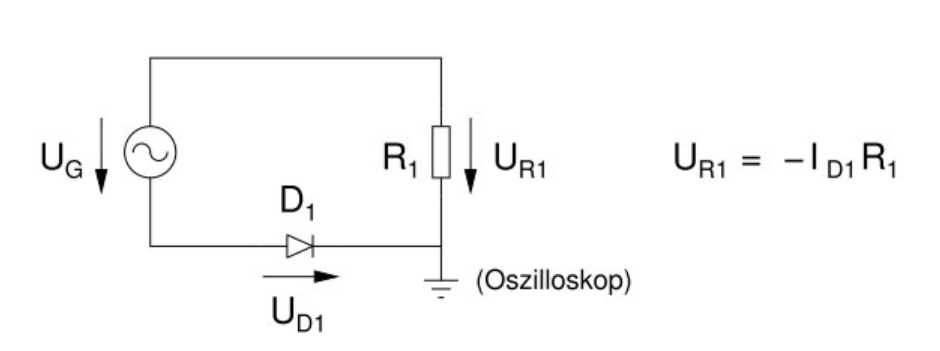
\includegraphics[width=150mm]{diodenschaltung.png}
  \caption{Diodenschaltung}
  \label{Figure8.3.1}
\end{figure}

\subsection{Durchführung}
Die Schaltung wird gemäß Plan zuerst mit einer roten LED und dann mit der 1N4148 Diode zur Vergleichsmessung in Serie mit einem $100\Omega$ Widerstand aufgebaut. Kanal 1 des Oszilloskops misst die Spannung an der Diode, Kanal 2 die Spannung am Widerstand (muss aufgrund der Position der Erdung invertiert geschalten werden). Das Oszilloskop befindet sich im XY-Betrieb, wodurch die Kennlinie sichtbar wird. Die Durchlassspannung wird mittels Cursor gemessen.

\subsection{Ergebnis}
Die Spannug wird mit Kanal 1 (X-Achse) an der Diode gemessen, der Strom mit Kanal 2 (Y-Achse) am Widerstand. Das Oszilloskop kann eigentlich nur Spannungen Messen, da der Strom jedoch über den Widerstand direkt proportional zur Spannung ist, kann dieser leicht berechnet werden. Um eine gute Darstellung der Kennlinie zu erreichen, muss eine geeignete Skalierung der Y-Achse eingestellt werden. Wenn die Durchlassspannung erreicht ist, kann viel Strom fließen.

\begin{figure}[H]
  \centering
  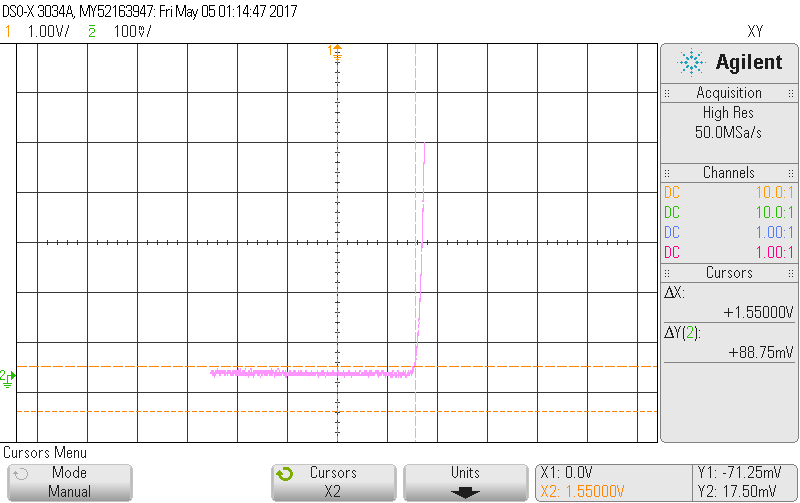
\includegraphics[width=150mm]{kennlinie_led.png}
  \caption{Kennlinie LED rot}
  \label{Figure8.5.1}
\end{figure}

Die Durchlassspannung der roten LED liegt laut Cursormessung bei $1,55V$. Diese ist etwas höher als bei \"herkömmlichen\" Dioden (siehe unten), da mit niedrigeren Spannungen kein sichtbares Licht erzeugt werden kann.

\begin{figure}[H]
  \centering
  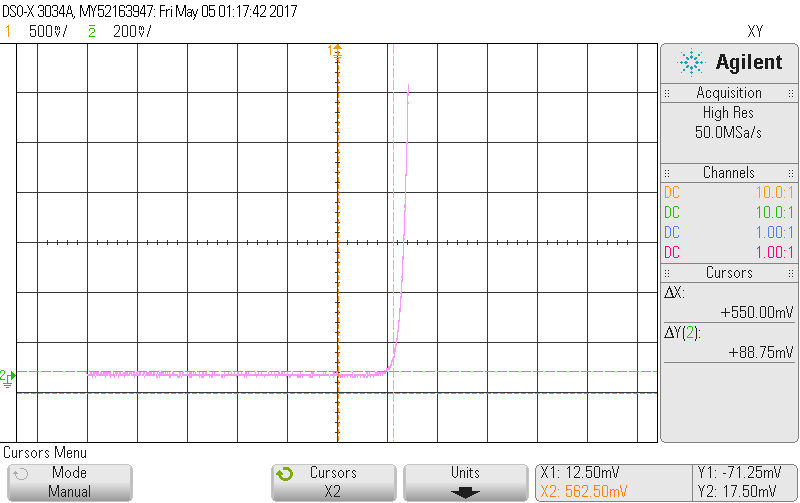
\includegraphics[width=150mm]{kennlinie_1n4148.png}
  \caption{Kennlinie 1N4148}
  \label{Figure8.5.2}
\end{figure}

Die Durchlassspannung der 1N4148 Diode liegt laut Cursormessung bei $0,55V$.

\end{document}
